\scanpage{18}

\begin{center}
\uline{ACADÉMIE D'AIX-MARSEILLE}\\
INSPECTION ACADÉMIQUE\\
\uline{DE VAUCLUSE}
\end{center}

\figure{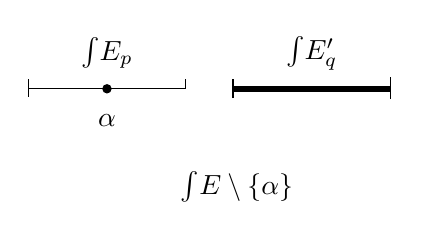
\begin{tikzpicture}[x=1cm,y=1cm]
\draw (0,0)--(2,0);\draw (0,-.10)--(0,.12);\draw (2,0)--(2,.13);\fill (1,0) circle (.06);
\node at (1,.45) {$\unsure{\int}E_p$};\node at (1,-.40) {$\alpha$};
\draw[line width=2pt] (2.6,0)--(4.6,0);\draw (2.6,-.12)--(2.6,.12);\draw (4.6,-.13)--(4.6,.15);
\node at (3.6,.45) {$\unsure{\int}E'_q$};
\node at (2.65,-1.25) {$\unsure{\int}E\setminus\{\alpha\}$};
\end{tikzpicture}}
\margin{$\unsure{p\geq}$}
\margin{278}

\deleted{
\[
F=\varinjlim_{A/F}\alpha\qquad G=\varinjlim_{A/G}\beta
\]
\[
\begin{aligned}
F\times G&=\varinjlim_{A/F}\underbrace{\alpha\times G}_{\varinjlim_{A/G}\alpha\times\beta}\\
&=\varinjlim_{A/F\times A/G}\alpha\times\beta
\end{aligned}
\]
\margin{$\alpha-F\qquad\beta-G$}
\[
\boxed{\begin{gathered}
\varphi_!(F\times G)=\varinjlim_{A/F\times A/G}
\underbrace{\varphi_!(\alpha\times\beta)}_{\varphi_!(\alpha)\times\varphi_!(\beta)}\\
\varphi_!(F)=\varinjlim_{A/F}\varphi_!(\alpha)\\
\varphi_!(G)=\varinjlim_{A/G}\varphi_!(\beta)
\end{gathered}}
\]
\diagram{\begin{tikzcd}[ampersand replacement=\&]
A\arrow[r,dash,"\varphi"]\&\mathcal X
\end{tikzcd}}
\diagram{\begin{tikzcd}[ampersand replacement=\&]
C=\mathcal X\arrow[r,shift right=2,"\unsure{u}=\varphi^*"']\&C'=\widehat A\arrow[l,shift right=2,"\unsure{v}=\varphi_!"']
\end{tikzcd}}
\figure{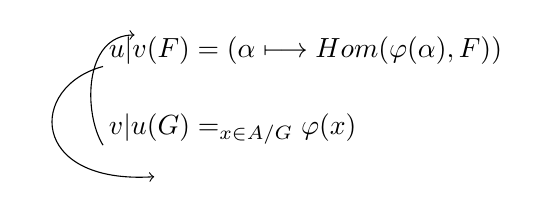
\begin{tikzpicture}
\node[anchor=west] at (0,0) {$\unsure{u|v}(F)=(\alpha\longmapsto\operatorname{Hom}(\varphi(\alpha),F))$};
\node[anchor=west] at (0,-1) {$\unsure{v|u}(G)=\varinjlim_{x\in A/G}\varphi(x)$};
\draw[->] (.05,-.2)..controls(-.9,-.45)and(-.9,-1.7)..(.7,-1.6);
\draw[->] (.05,-1.2)..controls(-.2,-.8)and(-.2,.2)..(.45,.2);
\end{tikzpicture}}
\margin{$u$ continu\\$v$ cocontinu}
\diagram{\begin{tikzcd}[ampersand replacement=\&,row sep=small]
\mathcal X\arrow[r]\&\widehat A\\
Y\&/\;a_i\to\varphi^*(Y)
\end{tikzcd}}
\diagram{\begin{tikzcd}[ampersand replacement=\&]
\varphi(a_i)\arrow[r]\&Y
\end{tikzcd}}
}

\margin{17}
